\chapter{Introduction}
\section{Motivation}
    \label{sec:motivation}
    % Explain why the thesis is written. How will it contribute and what is the current status of things in the field.
    This master's thesis is a collaboration between the Innovative Immersive Technologies for Learning (IMTEL) VR lab an the Department of Geography, both at NTNU. The project is a continuation of the Specialisation Project \emph{Immersive Virtual Field Trip for Field Course in Physical Geography}\cite{specialisation}, further described in \cref{sec:specialisation}.
    
    Field trips are an important part of many courses, especially in nature studies. There are however many limitations, and they are generally costly and time intensive to perform. Virtual field trips (VFTs) can help to get the most out of the field trips, for example by aiding students to prepare. Virtual field trips can also offer an alternative to people who are hindered from attending actual field trip (AFT).
    
    The field trip in question is for the course \emph{GEOG - 2012 Field Course in Physical Geography} at Norwegian University of Science and Technology (NTNU). The course is an introduction to the geography field, teaching students about different land formations and concepts, and how they are created\cite{geog2012}. The course also focuses on preparing, planning and executing an excursion. The field trip is a two-hour drive from Trondheim and lasts from a Monday morning to Wednesday afternoon. During this period the students spend about 10 hours in the field in addition to a separate excursion on the Tuesday. A lot of preparation is needed both before and during the field trip, and there are expenses related to transporting and housing the students for the duration of the trip.
    
    There already exists several virtual field trips, like Google Expeditions\cite{google_expeditions} where an educator can guide others through images. There are also applications using more advanced interaction, like the Climate Quest\cite{bachelor} application from NTNU where the user have to outrun a rising ocean level while shooting objects that are bad for the climate.
    %The new \emph{Oppdal Application} will, like Climate Quest, trading scalability for immersion. It will however focus on more on providing an opportunity to explore and learn, instead of invoking feelings around a topic.
    A new application was created, combining a virtual field trip with more advanced interaction. It was named the \textbf{\ApplicationName}. This application will, like Climate Quest, trade scalability for immersion, meaning it will need more advanced equipment. It will focus more on providing an opportunity to explore and learn, instead of invoking feelings around a topic like the Climate Quest. The \ApplicationName \hspace{0.1cm} will be developed using \emph{open source} resources, meaning they will be free to use.
    
    As virtual field trip applications is an established term, there is also existing research on this subject. One of the leading sources of the research is Penn State University\cite{penn_state}. From a news article at Hypergrid Business\cite{hypergrid} the research is summarised as collecting data on both actual- and virtual field trips, concluding that students are very positive the Virtual Field Trips. In an article from Penn State in 2017, Klippel and others\cite{developing_and_evaluating} evaluated the current development of VR field trips. They found that many earlier barriers had been overcome and that VR technology was ready to become more prominent in the market. Their research is however centred Virtual Field Trips where interaction is mostly limited to looking around inside 360$^{\circ}$ images. The focus of this master's thesis is therefore to combine images with a reconstructed landscape and introduce more interaction with the virtual world.
    
\section{Stakeholders and Target Audience}
    The identified \textbf{stakeholders} for the master's project are as follows:
    
    \todo{Is sensors the right word?}
    
    \begin{itemize}
        %\item \textbf{Sensors} \\
        %In the end the master's project is to be graded, and it is designed for the students to show they are capable of performing a research project. Because of this the direction of the project and the quality of the report focus on proving this.
        
        \item \textbf{Scientific Community and General Public}\\
        In order to give the best possible contribution to the scientific community, the project has focused on following the norms and best practices of research. The project is also meant to contribute to the general public, both indirectly through the research and directly by the creation of the app for those who want to visit field trip area.
        
        \SPACE
        
        \item \textbf{Institute of Geography} \\
        As the main collaborator on the project, the Institute of Geography helps guide the learning outcome of the project. As the eventual owners of the application, they also provide input when prioritising features for the application.
        
        \SPACE
        
        \item \textbf{IMTEL} \\
        The developed applications are to be specific in content, but developed using general and customizable components. Some of these components can then be added to IMTEL's collection of general scripts to improve future development. This draws focus the code quality of the master's project.
    \end{itemize}
    
    The \textbf{target audience} of the \ApplicationName are the students of GEOG - 2012 Field Course in Physical Geography. This is an introduction course focusing on planning and performing a field course. The academic content included in the application can therefore be on a level where everyone trying it can learn something about the physical geography in the Vekveselva area.

\section{Research Questions}
    % Can iVFT contribute to better learning for a course with field trip?
    The research of this project will be centred around developing and testing the \textbf{ \ApplicationName}. LiDAR, a type of laser scanning, will be used to recreate a topological model of the area. Stereoscopic 360 images will be included to show the actual landscape and gameplay elements will be included to motivate and educate the users. The \ApplicationName \hspace{0.1cm} should originally be compared to a simpler, more scaleable application supplied by Penn State university, using the same images.
    
    %The research questions are based on those found in the Specialisation Project\cite{specialisation}, but have been improved and further explained.
    The research questions are based on the current literature on the topic of virtual field trips, and have been constructed to further investigate certain aspects or look at different perspectives. The research questions are based on those found in the Specialisation Project \cite{specialisation}, but have been edited as the project have unfolded. They have also been accompanied by explanations to make them clearer. The research questions are:
    
    \todo{Be open about changes, or restructure?}
    
    \SPACE
    
    \begin{itemize}
        \item \textbf{R1 - } \emph{Can a Virtual Field Trip be valuable as a support tool for courses with field trips?}
        
        Contributing to the current research on the field, the goal is to investigate how useful a Virtual Field Trip can be as a supportive learning tool to a university course.
        
        \SPACE
        
        \item \textbf{R2 - } \emph{Can the use of gameplay interaction elements in a Virtual Field Trip lead to a better learning outcome than applications based on displaying images?}
        
        Expanding on the current research on the field, this will focus on comparing an application with little interaction, to one with more to see if there are differences in how well they work.
        
        \SPACE
        
        \item \textbf{R3 - } \emph{What game design theories apply and should be used in a Virtual Field Trip application?}
        
        As the goal is to investigate if a more interactive application can provide a better learning outcome, it is important to chose the right kind of interactivity. This will be done by reading appropriate literature to determine which elements that best improve the experience. 
        
        \SPACE
        
        \item \textbf{R4 - } \emph{How can a Virtual Field Trip be developed?}
        
        What are the tools and methods required for developing a Virtual Field Trip? Is it possible to automate parts of the process?
    
        \SPACE
        
        % \item \textbf{R5 - } \emph{How does an omnidirectional treadmill compare to other ways of movement in VR?}
        
        % What are the pros and cons of this kind of input, especially for VR sickness and spatial awareness?
        
        \item \textbf{R5 - } \emph{Are virtual field trips exclusive for field of study?}
        
        The \ApplicationName \hspace{0.1cm} is developed with students from geography as its target audience. Is it possible, or a good idea, to broaden the content enough for it to be used by the general population?
    \end{itemize}
    
    
    \todo{Is R5 out of scope? Can it be commented on using only observation and 2-3 extra questions in questionnaire, or does it require a completely different test setup?}

\section{Research Method}
    % Create two applications and test them, use interviews with domain experts, and interviews and questionnaires with students that will take the course (and have taken it?).
    % Use development method with quantitative and qualitative evaluation
    Oates'\cite{research} Model of the Research Process is used to describe how this master's thesis is conducted. Simplified, Oates' model describes the research process divided into seven main parts, as seen in \cref{fig:oates}:
    
    \FloatBarrier
    \begin{figure}[htbp]
        \centering
        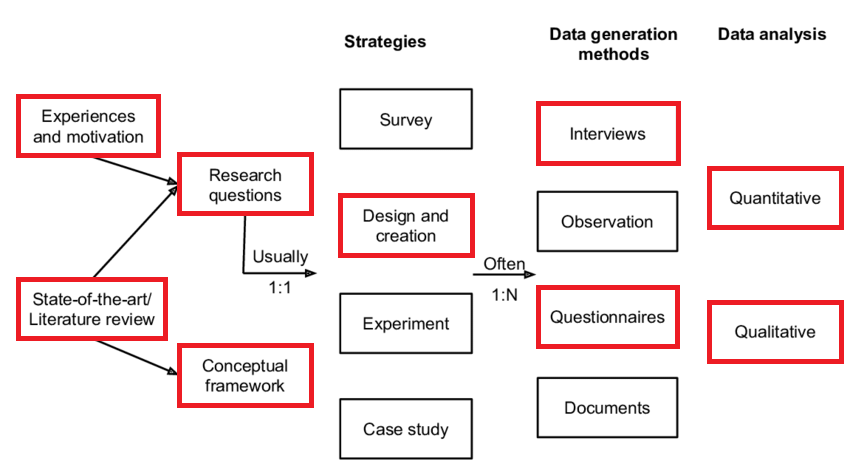
\includegraphics[width=\ImageWidth]{figures/oates_highlighted.png}
        \caption{Oates' Model of the Research Process}
        \label{fig:oates}
    \end{figure}
    \FloatBarrier
    
    The four first parts of the research process are stated to be more or less the same for all types of research. These are the four ''boxes'' to the left of \cref{fig:oates}: Experiences and motivation, Research questions, State-of-the-art/Literature review and Conceptual framework. The personal experience and motivation combined with a literature review create the research questions. The literature review also leads to the conceptual framework that \emph{''makes explicit how you structure your thinking about your research topic and the process undertaken''}. The remaining three categories have elements that can differ depending on the type of research. As indicated in the figure, one research question typically leads to one strategy, whereas a strategy can lead to several methods of data generation.
    
    \SPACE
    
    \subsection*{Research Method of this Master's Thesis}
    The research method was identified in the Specialisation Project\cite{specialisation}. This master's thesis conforms with Oates' model, with the four first parts present. This means that the project starts with existing experiences and motivation from the author. Combined with the literature review of the topic, research questions can be made. Additionally the conceptual framework of the terminology and relations take form and will be present throughout the thesis. The \textbf{Design and Create} strategy will be used to answer all of the presented research questions. This is done by developing the application, allowing it to be tested and compared to other applications.
    %Three data generation methods arise from the strategy: \textbf{Interviews}, \textbf{Observation} and \textbf{Questionnaires}. Students of the relevant course and domain experts will be invited to test the application. During these tests the users will be observed, then answer questionnaires and/or interviews.
    Two data generation methods arise from the strategy: \textbf{Interviews} and \textbf{Questionnaires}. People with VR equipment will be invited to download and test the \ApplicationName, whereas people without VR equipment will be supplied a video demonstrating the application. This video focused on showing the application as-is without explaining anything around it. This was to potentially uncover if anything in the application was unclear.
    Finally, the data analysis approach will be both \textbf{Qualitative} and \textbf{Quantitative}. The Questionnaires will be the main data source for the quantitative data analysis, whereas the interviews will supply data for the qualitative data analysis.
    
    \subsubsection{Questionnaire}
        The questions for the questionnaire were based on several other questionnaires with similar goals. Questions about individual differences, learning and enjoyment were taken from a study from Penn State in 2019 comparing the effect of virtual field trips to a control group \cite{transforming_earth_science}. Questions about control and active learning, and perceived learning effectiveness were taken from a study from 2010 investigating how desktop virtual reality enhances learning \cite{desktop_virtual_reality}. Questions about opinions on virtual field trips were taken from another Penn State paper from 2019 investigating virtual field trips in a geoscience course with elevated 360 degree images. The idea behind combining these questions is thoroughly investigate the learning and opinion aspect of the virtual field trip. The questions were used with a five point Likert scale \cite{likert} to create a quantitative and standardised data set.
        
        In addition to questions about learning, the System Usability Scale (SUS) \cite{sus} was used. This a relatively simple, but effective way of testing the usability of a system, using ten questions answered with a Likert scale. Questions from the User Experience Questionnaire (UEQ) \cite{ueq_questionnaire} were also included. These questions were meant to evaluate the application itself, not necessarily it's usefulness as a learning tool. The questionnaire can be viewed in \todo{import and reference questionnaire}.
        
    
    \subsubsection{Interview}
        The questions for the semi-structured interview were not taken from any literature, but created to find qualitative answers to the research questions. The questions were about evaluating the app itself and about virtual field trips and their possible usage in education. The questions for the interview can be viewed in \todo{import and reference interview}.

\section{Data Handling}
    % GDPR and group application from NSD
    % Questionnaire
    % Semi-structured interview
    When performing user tests, the data handling needs to be in accordance with the General Data Protection Regulation (GDPR)\cite{gdpr_eu}. In order to make sense of the regulations an article from \texttt{medium.com} detailing best practices of data handling was used. Following these practices, as little sensitive information as possible was collected. For the general questionnaires this meant none, focusing the questions on the application. The questions about the testers were also generalised, e.g. by placing them in age groups instead of asking for age. The questionnaire also avoided text answers, as this can be regarded as sensitive information.
    %For the semi-structured interviews, some personal information had to be kept. The practice of as-little-as-possible was still followed, and the interviews were recorded on non-internet connected devices, transcribed and anonymised.
    A group application was sent to the Norwegian Centre for Research Data to allow the collection of this data. 
    
    \todo{Update data handling after data has actually been handled}
    
    \begin{comment}
    \subsection*{Questionnaire}
        %The questionnaire was constructed to check which of the two applications the user tested and whether or not they had also tested the other.
        The questionnaire was constructed to check whether the tester had used the
        The users were also asked about their knowledge gain and how well they learned the area after using the application. Some questions from a short user experience questionnaire, provided by \texttt{ueq-online.org}\cite{ueq_questionnaire}, was used to assess the user experience of the applications. A question to investigate VR sickness was also added. The questionnaires were created using Google Forms\cite{google_forms}.
        %Online questionnaires have the issue of potentially logging the IP address of the user. This was circumvented by using one laptop for all the users, ensuring that IP addresses could not be linked to the answers. The questionnaire was also printed out to allow multiple users to answer at the same time. These questionnaires were then later added to the same database as the online questionnaire.
        
        \todo{Add questionnaire to appendix and cref}
        \todo{Avoided writing parts because of data handling}
    
    \subsection*{Semi-structured Interview}
    \end{comment}
        
\section{Changes due to Unforeseen Events}
    In the spring of 2020, the COVID 19 virus led to social distancing. This caused some changes to be made to the both the project and the application:
    
    \begin{itemize}
        \item \textbf{Testing} had to be done remotely instead of at the VR lab. The app had to be tested by however had VR equipment at home. Additionally a video demonstrating the application could be sent out to get feedback from those without VR equipment, especially students that attended the field trip in the autumn of 2019.
        
        \item \textbf{Focus} of the project had to be shifted from comparing two applications to evaluating one. This was because of the small possibility of people having two kinds of headsets available at home, the challenge of properly showing the differences via video, as well as reducing the extra work load introduced by the changes.
        
        %\todo{Other reasons? Possibility to capture footage from Oculus Go and make video?}
        
        \item \textbf{Teleporting} was added as an alternative way of movement in the \ApplicationName. This was to make it easier for home testing, both in development and evaluation, as very few people have a Virtuix Omni home.
        
        \item \textbf{Research questions} had to be changed late in the project. This mainly lead to removing a research question about how well the Virtuix Omni omnidirectional treadmill worked, as access to the lab was restricted. A new research question, R-5, was also added because of the changes to testing. By sending out a video and questionnaire, a broader audience was the data source, allowing to look at different opinions between geography students and the rest.
    \end{itemize}
    
    The changes also lead to delays in the progress plan, which will be discussed further in \todo{reference discussion: plan}.
    